\chapter{Approach}\label{cha:approach}

\section{Feature detection}\label{sec:feature_detection}

For feature detection, we used the approach, proposed
by~\cite{geigerAutomaticCameraRange2012} (see
\cref{sec:boards_features_detection,sec:classifier}).

\section{Camera calibration}\label{sec:camera_calibration}

In this work, we obtained the camera calibration in two steps: first, we
used the approach, proposed by~\cite{scaramuzzaToolboxEasilyCalibrating2006} to
obtain the initial approximation of the camera parameters. Then, we used
optimization to minimize the reprojection error between the board and the
back-projected corners. A division model is very powerful and can
express a wide range of distortions
\citep{prittsMinimalSolversRectifying2021}. In this work, we used a model with
two parameters to allow for better flexibility during the optimization.

\subsection{Reprojection error}\label{sub:reprojection_error}

The reprojection error is the distance between the reprojected point and the
measured one. It is used to evaluate the quality of the camera calibration.

We minimized the reprojection error between the board and back-projected
corners, which were initially detected. The projection and back-projection are
the inverse of each other, hence minimizing the error between the projection of
the board and the detected corners and minimizing the error between the
back-projection of the detected corners and the board are
equivalent. We minimized the error
between the board and the back-projected corners because back-projection does
not require the root finding.

Let's define the following variables: \(\boldsymbol{\theta} = \begin{pmatrix}
	\theta_x, \theta_y, \theta_z
\end{pmatrix}^{T}\) is the vector of Euler rotation angles, \(\mathbf{t} = \begin{pmatrix}
	t_x, t_y, t_z
\end{pmatrix}^{T}\) is the translation vector, \(\boldsymbol{\lambda} = \begin{pmatrix}
	\lambda_1, \lambda_2
\end{pmatrix}^{T}\) is the intrinsic parameters vector, \(\) is the focal
length, and \(\mathbf{s} = \begin{pmatrix}
	s_x, s_y
\end{pmatrix}^{T}\) is the sensor size.
From the input image, we know the resolution \(\mathbf{r} = \begin{pmatrix}
	r_x, r_y
\end{pmatrix}^{T}\).
From the rotation vector, we can compute the rotation matrix \(\mathbf{R}\) as:

From \(\boldsymbol{\theta}\), the rotation matrix $R$ can be calculated as follows:

\begin{equation}
	R = R(\theta_x) R(\theta_y) R(\theta_z),
\end{equation}

where

\begin{align}
	% R_x(\phi)   & =
	% \begin{bmatrix}
	% 	1 & 0          & 0           \\
	% 	0 & \cos(\phi) & -\sin(\phi) \\
	% 	0 & \sin(\phi) & \cos(\phi)
	% \end{bmatrix} \\
	% R_y(\theta) & =
	% \begin{bmatrix}
	% 	\cos(\theta)  & 0 & \sin(\theta) \\
	% 	0             & 1 & 0            \\
	% 	-\sin(\theta) & 0 & \cos(\theta)
	% \end{bmatrix}                 \\
	% R_z(\psi)   & =
	% \begin{bmatrix}
	% 	\cos(\psi) & -\sin(\psi) & 0 \\
	% 	\sin(\psi) & \cos(\psi)  & 0 \\
	% 	0          & 0           & 1
	% \end{bmatrix}
	R(\theta_x) & =
	\begin{bmatrix}
		1 & 0              & 0               \\
		0 & \cos(\theta_x) & -\sin(\theta_x) \\
		0 & \sin(\theta_x) & \cos(\theta_x)
	\end{bmatrix} \\
	R(\theta_y) & =
	\begin{bmatrix}
		\cos(\theta_y)  & 0 & \sin(\theta_y) \\
		0               & 1 & 0              \\
		-\sin(\theta_y) & 0 & \cos(\theta_y)
	\end{bmatrix} \\
	R(\theta_z) & =
	\begin{bmatrix}
		\cos(\theta_z) & -\sin(\theta_z) & 0 \\
		\sin(\theta_z) & \cos(\theta_z)  & 0 \\
		0              & 0               & 1
	\end{bmatrix}.
\end{align}

Then, \(H\) is given by:
\begin{equation}
	H = \begin{bmatrix}
		\mathbf{r_1} & \mathbf{r_2} & \mathbf{t}
	\end{bmatrix}.
\end{equation}

We can compute the intrinsic camera matrices as follows:
\begin{equation}
	K = \begin{bmatrix}
		\frac{f r_x}{s_x} & 0                 & \frac{r_x}{2} \\
		0                 & \frac{f r_y}{s_y} & \frac{r_y}{2} \\
		0                 & 0                 & 1
	\end{bmatrix}.
\end{equation}

Then, the back-projection of a 2D point \(\mathbf{u} = \begin{pmatrix}
	u, v, 1
\end{pmatrix}\) into a scene point with \(z = 0\) \(\mathbf{x} = \begin{pmatrix}
	x, y, 1
\end{pmatrix}\) is given by:
\begin{equation}
	\mathbf{x} = H g_{\lambda_1, \lambda_2}(K^{-1} \mathbf{u}).
\end{equation}

\subsection{Initial approximation}\label{sub:initial_approximation}

\cite{scaramuzzaToolboxEasilyCalibrating2006} proposed an automatic method for
camera calibration, which consisted of the following steps:
\begin{itemize}
	\item Solving for the camera extrinsic parameters
	\item Solving for the camera intrinsic parameters
	\item Linear refinement of the intrinsic and extrinsic parameters
	\item Iterative center detection
	\item Non-linear refinement
\end{itemize}

In this work, we focused on a single image, while the original approach relied
on multiple images. Therefore, we used only the first two steps of the
algorithm.

\subsubsection{Solving for the camera extrinsic parameters}\label{ssub:solving_for_the_camera_extrinsic_parameters}

To derive the solver for the camera extrinsic parameters, start from
\cref{eq:projection}:
\begin{align}
	\alpha \mathbf{u}                                                          & = K f(H\mathbf{x})       \\
	\alpha K^{-1} \mathbf{u}                                                   & = f(H\mathbf{x})    &  &
	\text{Move \(K\) to the left side}                                                                    \\
	\alpha g( K^{-1}\mathbf{u})                                                & = g(f(H\mathbf{x})) &  &
	\text{Set \(\mathbf{\widehat{u}} = K^{-1}\mathbf{u}\); apply \(g(\cdot)\) to both sides}              \\
	\alpha \begin{pmatrix}
		       \widehat{u}_x \\ \widehat{u}_y \\ \psi(r(\mathbf{\widehat{u}}))
	       \end{pmatrix}^{T} & = H\mathbf{x}.
\end{align}

For \(K\) we used the placeholder values.\ \(f\) was set to a constant value for
the typical consumer camera, and \(c_x, c_y\) were set to the center of the
image.
The correct values will be computed during the optimization \cref{sub:optimization}.

To eliminate the dependency on the scale \(\alpha\), multiply both sides
vectorially by \(g(\mathbf{\widehat{u}})\):
\begin{equation}
	\alpha g(\mathbf{\widehat{u}}) \times g(\mathbf{\widehat{u}})
	= g(\mathbf{\widehat{u}}) \times H\mathbf{x}
	= 0 \implies
	\begin{pmatrix}
		\widehat{u}, \widehat{v}, \psi(r(\mathbf{\widehat{u}}))
	\end{pmatrix}^{T} \times \begin{bmatrix}
		\mathbf{r_1} & \mathbf{r_2} & \mathbf{t}
	\end{bmatrix}^{T} \mathbf{x} = 0
	\label{eq:eq_no_multiplier}.
\end{equation}

From \cref{eq:eq_no_multiplier}, we can see that a point contributes to three
homogeneous equations:
\begin{align}
	\widehat{v} (r_{31}x + r_{32} y + t_3) -
	g(r(\mathbf{\widehat{u}})) (r_{21}x + r_{22}y + t_2 ) & = 0
	\label{eq:scaramuzza_system_1}                              \\
	g(r(\mathbf{\widehat{u}})) (r_{11}x + r_{12}y + t_1) -
	\widehat{u} (r_{31}x + r_{32} y + t_3)                      & = 0
	\label{eq:scaramuzza_system_2}                              \\
	\widehat{u} (r_{21}x + r_{22}y + t_2 ) -
	\widehat{v} (r_{11}x + r_{12}y + t_1)                 & = 0
	\label{eq:scaramuzza_system_3}.
\end{align}

Only \cref{eq:scaramuzza_system_3} is linear in the unknowns. Each point gives a
single equation. Now, by rewriting the equation in the matrix form
\(M \cdot \mathbf{h} = 0\), where
\[
	\mathbf{h} = \begin{pmatrix}
		r_{11}, r_{12}, r_{21}, r_{22}, r_{31}, r_{32}
	\end{pmatrix}^{T},
\]
we get:
\begin{equation}
	M = \begin{bmatrix}
		-\widehat{v}_1 x_1 & -\widehat{v}_1 y_1 & -\widehat{u}_1 x_1 & -\widehat{u}_1 y_1 & -\widehat{v}_1 & -\widehat{u}_1 \\
		\vdots             & \vdots             & \vdots             & \vdots             & \vdots         & \vdots         \\
		-\widehat{v}_N x_N & -\widehat{v}_N y_N & -\widehat{u}_N x_N & -\widehat{u}_N y_N & -\widehat{v}_N & -\widehat{u}_N
	\end{bmatrix}
\end{equation}, where \(N\) is the number of points.

The linear estimate of \(\mathbf{h}\) is found by minimizing \(\left\lVert M \cdot
\mathbf{h} \right\rVert ^{2}\) using SVD. The solution is known up to a scale factor.

To find \(t_1\) and \(t_2 \), note that \(\mathbf{r_1}\) and
\(\mathbf{r_2}\) are orthonormal:
\begin{subnumcases}{}
	\lambda^{2} r_{11} r_{12} + \lambda^{2} r_{21} r_{22} + \lambda^{2} r_{31}
	r_{32}  = 0
	\label{eq:orthonormality_1}                                                     \\
	\lambda \sqrt{r_{11}^{2} + r_{21}^{2} + r_{31}^{2}}                            = 1
	\label{eq:orthonormality_2}                                                     \\
	\lambda \sqrt{r_{12}^{2} + r_{22}^{2} + r_{32} ^{2}}                            = 1
	\label{eq:orthonormality_3},
\end{subnumcases}
where \(\lambda\) is non-zero multiplier.

Now, to solve for \(r_{31}\) and \(r_{32} \), first find possible values for
\(r_{32} ^{2}\):
\begin{align}
	- \frac{r_{11} r_{12} + r_{21} r_{22}}{r_{32} }                         & = r_{31} &  &
	\text{Solve eq. (\ref{eq:orthonormality_1}) for \(r_{31}\)}
	\label{eq:orthonormality_4}
	\\
	\sqrt{\lambda^{2} \left( \frac{(r_{11} r_{12} + r_{21} r_{22})^{2}}{r_{32} ^{2}} +
	r_{11}^{2} + r_{21}^{2}\right)}                                      & = 1   &  &
	\text{Substitute into eq. (\ref{eq:orthonormality_2})}                            \\
	\lambda^{2} \left( \frac{(r_{11} r_{12} + r_{21} r_{22})^{2}}{r_{32} ^{2}} +
	r_{11}^{2} + r_{21}^{2}\right)                                       & = 1   &  &
	\text{Square both sides}                                                          \\
	\lambda^{2} \left(\frac{(r_{11} r_{12} + r_{21} r_{22})^{2}}{r_{32} ^{2}} +
	r_{11}^{2} + r_{21}^{2} - r_{12}^{2} - r_{22}^{2} - r_{32} ^{2} \right) & = 0   &  &
	\text{Subtract eq. (\ref{eq:orthonormality_3})}
	\label{eq:orthonormality_5}
	\\
	\frac{(r_{11} r_{12} + r_{21} r_{22})^{2}}{r_{32} ^{2}} +
	r_{11}^{2} + r_{21}^{2} - r_{12}^{2} - r_{22}^{2} - r_{32} ^{2}         & = 0   &  &
	\text{Divide both by \(\lambda ^{2}\)}                                            \\
	r_{32} ^{4} - (r_{11}^{2} + r_{21}^{2} - r_{12}^{2} -
	r_{22}^{2}) r_{32} ^{2} - (r_{11} r_{12} + r_{21} r_{22})^{2}           & = 0   &  &
	\text{Multiply by \(r_{32} ^{2}\)}
	\label{eq:orthonormality_6}.
\end{align}

Now, solve \cref{eq:orthonormality_6} for \(r_{32} ^{2}\), and take a root to find
possible values for \(r_{32} \).

To find \(r_{31}\), substitute the found values for \(r_{32} \) into
\cref{eq:orthonormality_4} or subtract \cref{eq:orthonormality_3} from
\cref{eq:orthonormality_2} and solve for \(r_{31}\) depending on the value
of \(r_{32} \):
\begin{subnumcases}{}
	r_{31}  = - \frac{r_{11} r_{12} + r_{21} r_{22}}{r_{32} } &
	\text{\(r_{32}  \neq 0\)} \\
	r_{31}  =  r_{11}^{2} + r_{21}^{2} - r_{12}^{2} - r_{22}^{2} &
	\text{\(r_{32}  = 0\)}.
\end{subnumcases}

Now, it's possible to find \(H\) for each of the pairs of \(r_{31}\) and
\(r_{32} \).

Lastly, to select the correct \(H\), the author assumes that one of the boards'
corners has the coordinates \( \begin{pmatrix}
	0, 0
\end{pmatrix}^{T}\). Then, the rotation wouldn't affect this
point, and it would be projected to   \(\begin{pmatrix}
	r_{31}, r_{32}
\end{pmatrix}^{T}\). Hence, the best matrix would be such that has the closest
\(\begin{pmatrix}
	r_{31}, r_{32}
\end{pmatrix}^{T}\) to \(\begin{pmatrix}
	x, y
\end{pmatrix}^{T}\) of the corner, which is associated with the board's corner
with coordinates \(\begin{pmatrix}
	0, 0
\end{pmatrix}^{T}\).

However, often the algorithm finds who matrices \(H\) such that they have the
same \(r_{31}\) and \(r_{32} \), but different \(r_{11}\), \(r_{21}\), \(r_{12}\). To
find the best matrix, we found the intrinsic values for each of them and
back-projected the board's corners using both matrices.
Then, we used the one which gave the smallest reprojection error.

\subsubsection{Solving for the camera intrinsic parameters}\label{subsub:solving_for_the_camera_intrinsic_parameters}

Now, to find the rest of the parameters, we substitute the values, found in the
previous step into \cref{eq:scaramuzza_system_1} and
\cref{eq:scaramuzza_system_2}. We assumed the number of the division model's
parameter to be equal to 2, and the scalar multiplier to be equal to 1
\cref{subsub:back_projection_using_the_division_model}:

\begin{equation}
	\begin{bmatrix}
		A_1 \rho_1^{2} & A_1 \rho_1^{4} & -v_1   \\
		C_1 \rho_1^{2} & C_1 \rho_1^{4} & -v_1   \\
		\cdots         & \cdots         & \cdots \\
		A_N \rho_N^{2} & A_N \rho_N^{4} & -v_N   \\
		C_N \rho_N^{2} & C_N \rho_N^{4} & -v_N
	\end{bmatrix} \cdot \begin{bmatrix}
		\lambda_1 \\
		\lambda_2 \\
		t_3
	\end{bmatrix} = \begin{bmatrix}
		B_1 - A_1 \\
		D_1 - C_1 \\
		\cdots    \\
		B_N - A_N \\
		D_N - C_N
	\end{bmatrix},
\end{equation}
where
\begin{align}
	A_i & = r_{21} x_i + r_{22} y_i + t_2  \\
	B_i & = v_i (r_{31} x_i + r_{32} y_i)  \\
	C_i & = r_{11} x_i + r_{12} y_i + t_1  \\
	D_i & = u_i (r_{31} x_i + r_{32} y_i).
\end{align}

The solution can be found using the least squares method.

\subsection{Optimization}\label{sub:optimization}

The loss function is the sum of the squared reprojection errors between the board and
the back-projected corners, which were initially detected:
\begin{equation}
	L = \sum_{i=1}^{N} \left\lVert
	H^{-1} g_{\lambda_1, \lambda_2}(K^{-1} \mathbf{u_i}) -
	\mathbf{x_i} \right\rVert^2.
\end{equation}

For the initial guess, we used the randomly chosen constant small values.

The model converged to the same results compared to the initial parameters, set
using the Scaramuzza solver, unless the initial guess was very degenerate (i.e.
\(R\) was such that the board plane passed through the principal point and all
back-projected points were projected onto the same line).

This issue also occurred with random small initial values, due to the best
approximation for \(R\) which minimizes \(L\) when the distance from the
back-projected board from measure one was high (i.e., the \(t\) was far from
the true value) being the degenerate solution. To avoid this issue, we first optimized only the \(t\),
until the loss function converged, meaning that \(t\) is close to the true
value.

However, another issue was that when the board was rotated close to the
\(180^{\circ}\), \(R\) once again converged to the degenerate solution. In order
to avoid this issue, we found the solution with the initial \(\theta_z\) set to
value, close to \(0^{\circ}\) and \(180^{\circ}\), and then used the solution
which minimized the loss function.

\section{Additional features detection}\label{sec:additional_features_detection}

Often, not all of the board's corners were detected initially. Firstly, we
assumed that the whole board was detected, and imputed the missing points in the
board space (\cref{fig:extended_board_img}). Then, we tried extending the board
points.

We used the obtained camera parameters to then project the imputed board points
into the image space.

\section{Classifier}\label{sec:classifier}

In this work, one of the methods we used was proposed by
\cite{geigerAutomaticCameraRange2012} as it didn't require the whole board to be
visible, automatically determines the board's number of rows and columns and
worked quite well on highly-distorted images.

In this work, we directly used the following steps from the algorithm:
\begin{enumerate}
	\item Corner detection
	\item Sub-pixel corner and orientation refinement
\end{enumerate}

\subsection{Corner detection}\label{sub:corner_detection}

% \begin{multicols}{2}
%
% 	According to \cite{geigerAutomaticCameraRange2012}, the following approach proved to be
% 	more robust to image clutter and blur than other common choices
% 	\citep{harrisCombinedCornerEdge1988, shiGoodFeaturesTrack2000}.
%
% 	To detect corners in a grayscale image $I$, the author used two $n \times n$ prototypes
% 	for axis-aligned and $45^{\circ}$ rotated corners, respectively.
% 	Each prototype
% 	is constructed using four filter kernels $\{A, B, C, D\}$. The corner likelihood
% 	$c$ at each pixel is computed by:
%
% 	\columnbreak
%
% 	\begin{figure}[H]
% 		\centering
%
% 		\begin{subfigure}{0.48\textwidth}
% 			\centering
% 			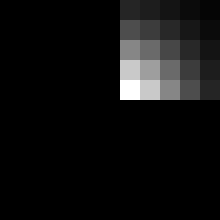
\includegraphics[width=0.23\textwidth]{./template_1_a.png}
% 			
\includegraphics[width=0.23\textwidth]{./template_1_b.png}
% 			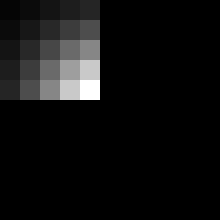
\includegraphics[width=0.23\textwidth]{./template_1_c.png}
% 			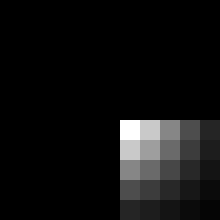
\includegraphics[width=0.23\textwidth]{./template_1_d.png}
% 			\caption{Corner prototype 1 (A, B, C, D)}
% 		\end{subfigure}
%
%     \vspace{0.5cm}
%
% 		\begin{subfigure}{0.48\textwidth}
% 			\centering
% 			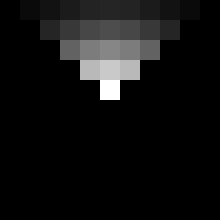
\includegraphics[width=0.23\textwidth]{./template_2_a.png}
% 			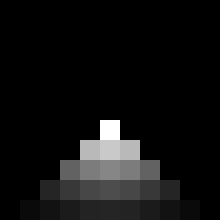
\includegraphics[width=0.23\textwidth]{./template_2_b.png}
% 			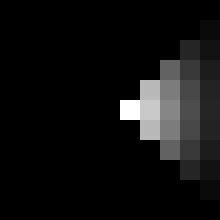
\includegraphics[width=0.23\textwidth]{./template_2_c.png}
% 			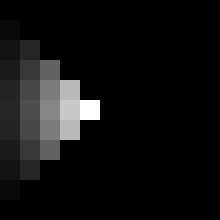
\includegraphics[width=0.23\textwidth]{./template_2_d.png}
% 			\caption{Corner prototype 2 (A, B, C, D)}
% 		\end{subfigure}
%
% 		\caption{Corner prototypes}
% 	\end{figure}
%
% \end{multicols}

\begin{figure}[h]
	\centering

	\begin{subfigure}{0.45\textwidth}
		\centering
		\begin{minipage}{\textwidth}
			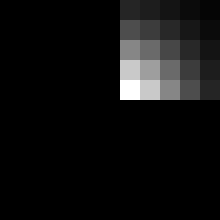
\includegraphics[width=0.24\textwidth]{./template_1_a.png}
			
\includegraphics[width=0.24\textwidth]{./template_1_b.png}
			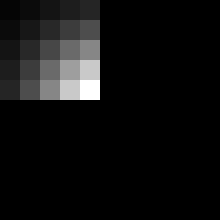
\includegraphics[width=0.24\textwidth]{./template_1_c.png}
			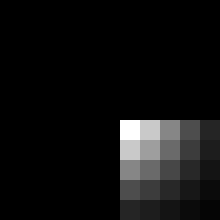
\includegraphics[width=0.24\textwidth]{./template_1_d.png}
		\end{minipage}
		\caption{Corner prototype 1 (A, B, C, D)}
	\end{subfigure}
	\hfill
	\begin{subfigure}{0.45\textwidth}
		\centering
		\begin{minipage}{\textwidth}
			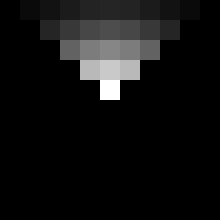
\includegraphics[width=0.24\textwidth]{./template_2_a.png}
			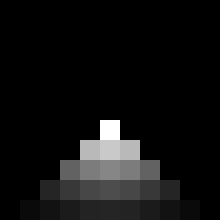
\includegraphics[width=0.24\textwidth]{./template_2_b.png}
			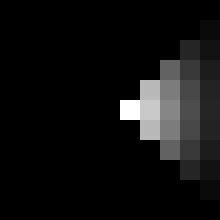
\includegraphics[width=0.24\textwidth]{./template_2_c.png}
			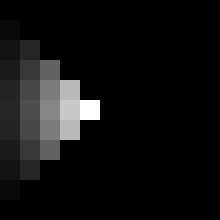
\includegraphics[width=0.24\textwidth]{./template_2_d.png}
		\end{minipage}
		\caption{Corner prototype 2 (A, B, C, D)}
	\end{subfigure}
	\begin{subfigure}{0.3\linewidth}
		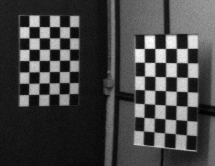
\includegraphics[width=\textwidth]{10.png}
		\caption{Input image}
	\end{subfigure}
	\begin{subfigure}{0.3\linewidth}
		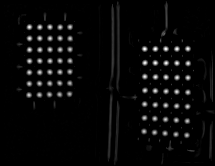
\includegraphics[width=\textwidth]{11.png}
		\caption{Corner likelihood}
	\end{subfigure}

	\caption{Corner prototypes \citep{geigerAutomaticCameraRange2012}}
	\label{fig:corner_prototypes}
\end{figure}

According to \cite{geigerAutomaticCameraRange2012}, the following approach proved to be
more robust to image clutter and blur than other common choices
\citep{harrisCombinedCornerEdge1988, shiGoodFeaturesTrack2000}.

To detect corners in a grayscale image $I$, the author used two $n \times n$ prototypes
for axis-aligned and $45^{\circ}$ rotated corners, respectively.
Each prototype
is constructed using four filter kernels $\{A, B, C, D\}$ (\cref{fig:corner_prototypes}). The corner likelihood
$c$ at each pixel is computed by:

\begin{equation}
	\begin{aligned}
		c     & =\max \left(s_1^1, s_2^1, s_1^2, s_2^2\right)                                             \\
		s_1^i & =\min \left(\min \left(f_A^i, f_B^i\right)-\mu, \mu-\min \left(f_C^i, f_D^i\right)\right) \\
		s_2^i & =\min \left(\mu-\min \left(f_A^i, f_B^i\right), \min \left(f_C^i, f_D^i\right)-\mu\right) \\
		\mu   & =0.25\left(f_A^i+f_B^i+f_C^i+f_D^i\right)
	\end{aligned}.
\end{equation}

Then, the authors apply the conservative non-maximum suppression to the
response map, and additionally filter the corners by assuring that there are two
modes of the gradient directions.

% \subsection{Sub-pixel Corner and Orientation Refinement}\label{sub:sub_pixel_corner_and_orientation_refinement}
%
% Sub-pixel accurate corner locations and edge orientations are refined using the following optimizations:
%
% For sub-pixel corner localization, the corner $\mathbf{c}$ in a 2D space
% $\mathbb{R}^2$ is refined using the assumption that the gradient direction
% \(\mathbf{g_{p}}\) at
% each pixel  \(\mathbf{p}\) in the small neighbourhood around the corner is
% orthogonal to \(\mathbf{p} - \mathbf{c}\).
%
% \begin{equation}
% 	\mathbf{c}=\arg \min _{\mathbf{c}^{\prime}} \sum_{\mathbf{p} \in
% 	\mathcal{N}_{\mathbf{I}}\left(\mathbf{c}^{\prime}\right)}\left(\mathbf{g}_{\mathbf{p}}^T\left(\mathbf{p}-\mathbf{c}^{\prime}\right)\right)^2
% \end{equation}
%
% For the orientation refinement, authors minimize the distance from the
% orientation vectors \(\mathbf{e_1}, \mathbf{e_2}\) to the gradient directions
% \(\mathbf{g_p}\) in the neighbourhood of the corner.
%
% \begin{equation}
% 	\mathbf{e}_i=\arg \min _{\mathbf{e}_i^{\prime}} \sum_{\mathbf{p} \in
% 		\mathcal{M}_i}\left(\mathbf{g}_{\mathbf{p}}^T \mathbf{e}_i^{\prime}\right)^2
% 	\quad \text { s.t. } \mathbf{e}_i^{\prime T} \mathbf{e}_i^{\prime}=1
% \end{equation}.

\subsection{Classifier training}\label{sub:classifier_training}

We tested the approach of \cite{geigerAutomaticCameraRange2012}, and,
alternatively, the Hessian responses for the image, as proposed by
\cite{chenNewSubPixelDetector2005}.

To create a training dataset, we collected the true and false positives from the
corners we already detected.

For each of the detected corners on all images, we collected the values of the
response function at the previously detected corners, and around them.
We didn't collect the values of all of the pixels, to reduce the number
of very simple examples.

To determine the threshold for the classification, we used the ROC curve, and
found the threshold which maximizes
the geometric mean of the true positive rate and the false positive rate.

We used both approaches to train the classifier and compared the
results in \cref{sec:classification}.

